%---------------------------------------------------------------------------
%	PACKAGES AND OTHER DOCUMENT CONFIGURATIONS
%---------------------------------------------------------------------------
\documentclass[final]{beamer}
\usepackage{gensymb}
\usepackage{textcomp}
\usepackage{overpic}
\usepackage[scale=1]{beamerposter} % Use the beamerposter package for laying out the poster
\usetheme{confposter} % Use the confposter theme supplied with this template
\setbeamercolor{block title}{fg=jblue,bg=white} % Colors of the block titles
\setbeamercolor{block body}{fg=black,bg=white} % Colors of the body of blocks
\setbeamercolor{block alerted title}{fg=white,bg=jblue} % Colors of the highlighted block titles
\setbeamercolor{block alerted body}{fg=black,bg=jblue!10} % Colors of the body of highlighted blocks
% Many more colors are available for use in beamerthemeconfposter.sty
%---------------------------------------------------------------------------
% Define the column widths and overall poster size
% To set effective sepwid, onecolwid and twocolwid values, first choose how many columns you want and how much separation you want between columns
% In this template, the separation width chosen is 0.024 of the paper width and a 4-column layout
% onecolwid should therefore be (1-(# of columns+1)*sepwid)/# of columns e.g. (1-(4+1)*0.024)/4 = 0.22
% Set twocolwid to be (2*onecolwid)+sepwid = 0.464
% Set threecolwid to be (3*onecolwid)+2*sepwid = 0.708
\newlength{\sepwid}
\newlength{\onecolwid}
\newlength{\twocolwid}
\newlength{\threecolwid}
\setlength{\paperwidth}{48in} % A0 width: 46.8in
\setlength{\paperheight}{36in} % A0 height: 33.1in
\setlength{\sepwid}{0.024\paperwidth} % Separation width (white space) between columns
\setlength{\onecolwid}{0.1386667\paperwidth} % Width of one column
\setlength{\twocolwid}{0.3013333\paperwidth} % Width of two columns
\setlength{\topmargin}{0.0in} % Reduce the top margin size
%---------------------------------------------------------------------------
\usepackage{graphicx}  % Required for including images
\usepackage{booktabs} % Top and bottom rules for tables
%---------------------------------------------------------------------------
%	TITLE SECTION 
%---------------------------------------------------------------------------
\title{Position-Free Monte Carlo Simulation for Arbitrary Layered BSDFs} % Poster title
\author{Yu Guo$^1$, Milo\v{s} Ha\v{s}an$^2$ and Shuang Zhao$^1$} % Author(s)
\institute{$^1$University of California, Irvine \hspace{2cm}
$^2$Autodesk Inc.\\
\vspace{1cm}
\Large{ACM Transactions on Graphics (SIGGRAPH Asia 2018), 37(6), 2018}} % Institution(s)
%----------------------------------------------------------------------------
\begin{document}
\addtobeamertemplate{headline}{}{
\begin{tikzpicture}[remember picture,overlay] 
\node [shift={(-10cm,-8cm)}] at (current page.north east) {
\includegraphics[height=9cm]{images/logo/SA2018_Logo1a.jpg}}; 
\end{tikzpicture}
\begin{tikzpicture}[remember picture,overlay] 
\node [shift={(-116cm,-8cm)}] at (current page.north east) {
\includegraphics[height=7cm]{images/logo/UCI.png}}; 
\end{tikzpicture}
\begin{tikzpicture}[remember picture,overlay] 
\node [shift={(-107cm,-8cm)}] at (current page.north east) {
\includegraphics[height=7cm]{images/logo/Autodesk.png}}; 
\end{tikzpicture}
}

\begin{frame}[t] % The whole poster is enclosed in one beamer frame
\vspace{-1.5cm}
\begin{columns}[t] % The whole poster consists of three major columns, the second of which is split into two columns twice - the [t] option aligns each column's content to the top
    %----------------------------------------------------------------------------
    %	LEFT
    %---------------------------------------------------------------------------
    \begin{column}{\sepwid}\end{column} % Empty spacer column
    \begin{column}{\twocolwid} % The first column
        \begin{block}{Introduction}
            \begin{figure}
                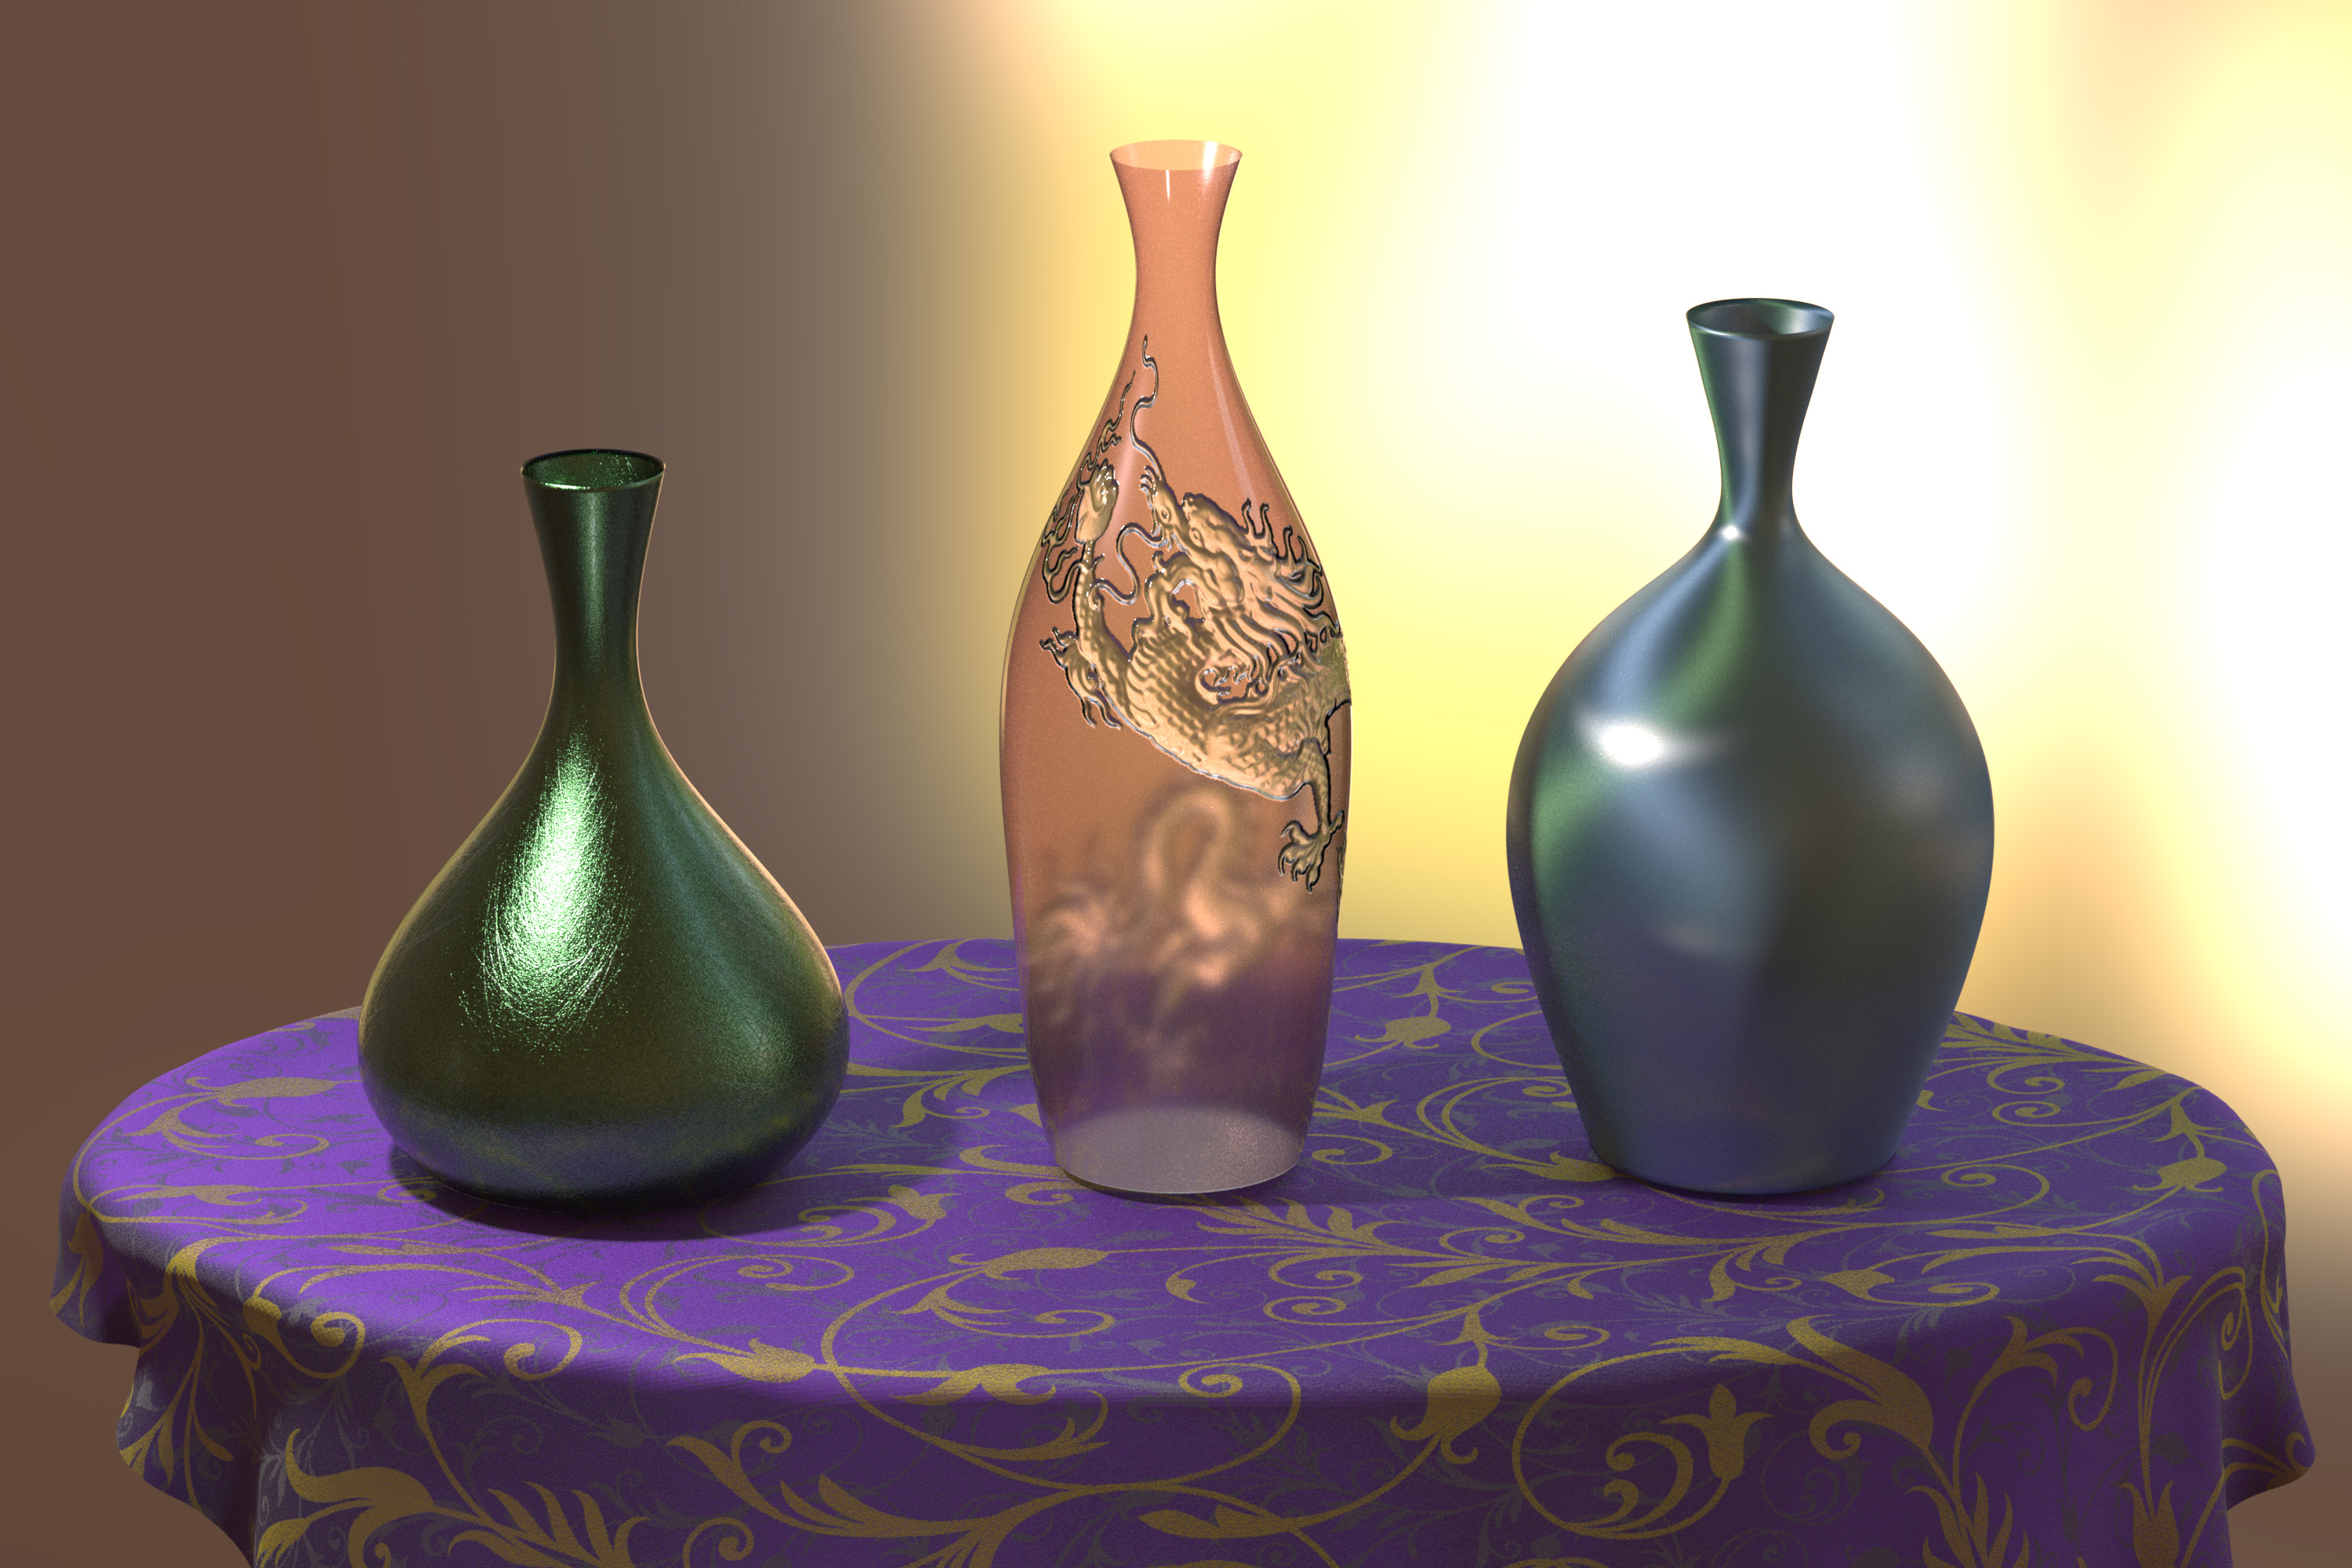
\includegraphics[width=0.9\linewidth]{images/teaser/teaser.jpg}
            \end{figure}
        
            \large{
            In this paper, we introduced a new BSDF model to capture the appearance of layered materials. 
            Inside the evaluation and sampling routines of the layered BSDF, we run a Monte Carlo simulation of light transport within flat slabs. 
            This is substantially faster than explicitly constructing the layer geometry, 
            but also allows constructing light transport paths that would not easily be available to a generic light transport algorithm, 
            due to our new position-free path formulation.
            
            \vspace{1cm}
            
            Within this framework, we introduced unbiased Monte Carlo techniques analogous to a forward path tracer with next event estimation (NEE) and a fully bidirectional estimator.
            We demonstrated the capabilities of our solution on a number of examples, featuring multiple layers with surface and volumetric scattering, surface and phase function anisotropy, and spatial variation in all parameters.
            This leads to the first BSDF layering solution that offers unbiased accuracy and full flexibility in setting the layer properties.
            }

        \end{block}
        
        \vspace{2cm}
        
        \begin{block}{Assumption}
            \begin{figure}
            	
\includegraphics[width=0.5\columnwidth]{images/illustration/assumption.pdf}
            \end{figure}
            \large{
            \textbf{Small displacement assumption:}
            Since the geometric thickness $h$ of the layer is small, we assume the displacements (e.g., $\Delta x$) of light's entrance and departure locations can be neglected.
            }
        \end{block}
    \end{column} % End of the first column
    
    %----------------------------------------------------------------------------
    %        MIDDLE
    %----------------------------------------------------------------------------
    \begin{column}{\sepwid}\end{column} % Empty spacer column
    \begin{column}{\twocolwid} % Begin a column which is two columns wide (column 2)
        \begin{block}{Methods}
            \textbf{BSDF sampling:}
            Forward path tracing in flat slab configuration
            
            \textbf{BSDF evaluation:}
            \begin{figure}
                \begin{tabular}{c}
                    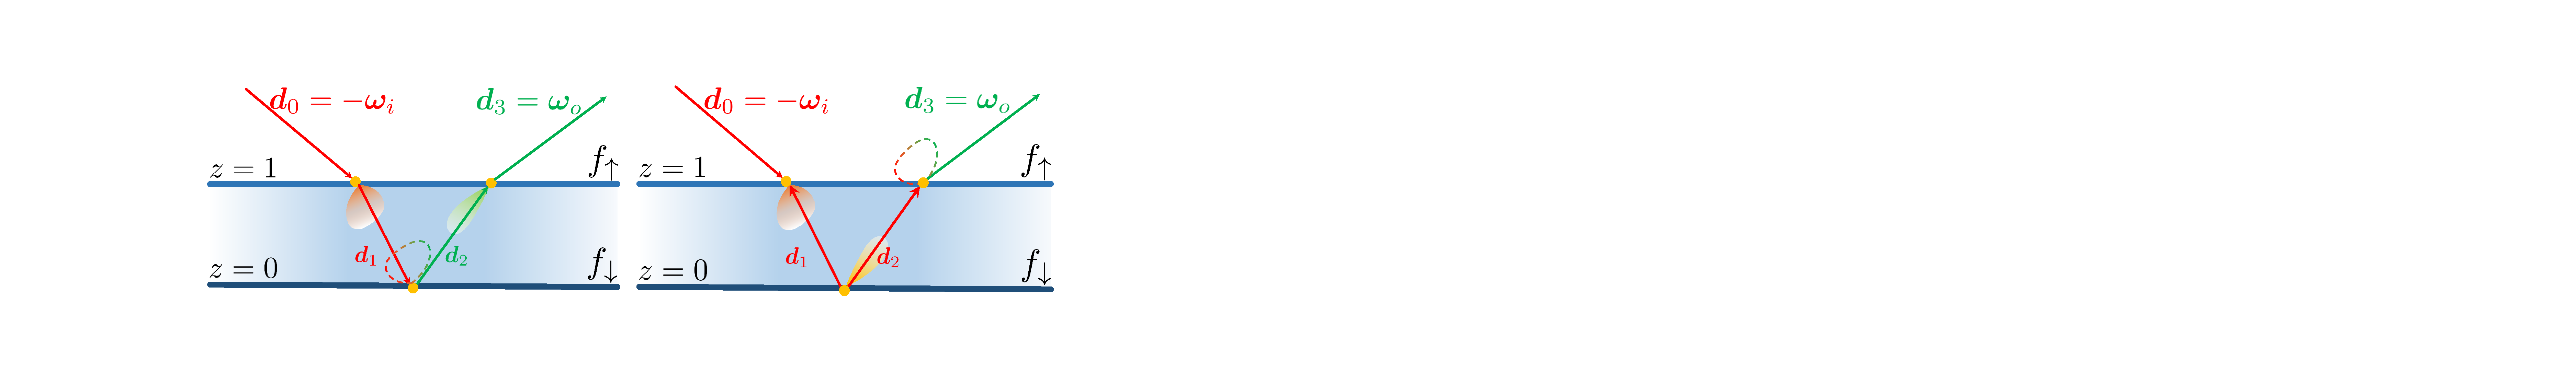
\includegraphics[width=0.6\textwidth]{images/illustration/unidir.pdf}\\
                    \small{Unidirectional estimator}
                \end{tabular}
            \end{figure}
            
            \begin{figure}
                \begin{tabular}{c}
                    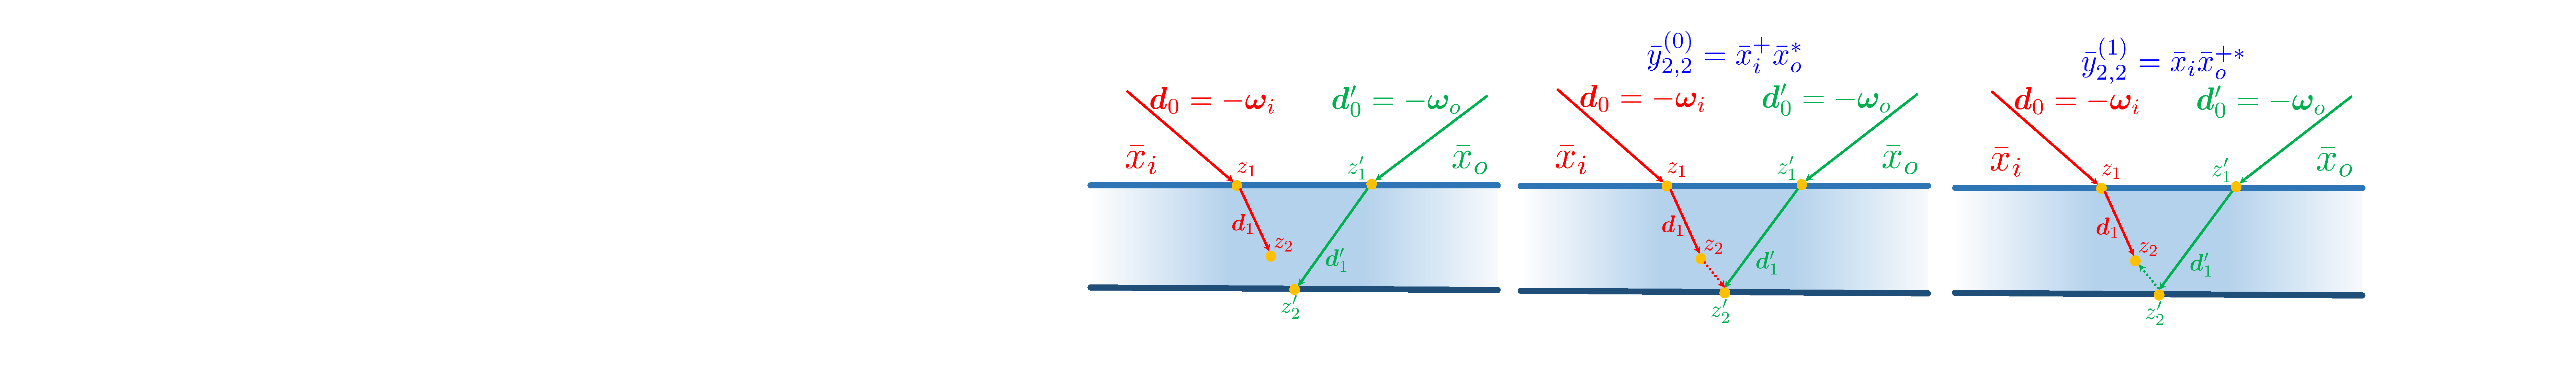
\includegraphics[width=0.9\textwidth]{images/illustration/bidir.pdf}\\
                    \small{Bidirectional estimator}
                \end{tabular}
            \end{figure}

            \textbf{Pdf estimation:}
            \begin{figure}
            	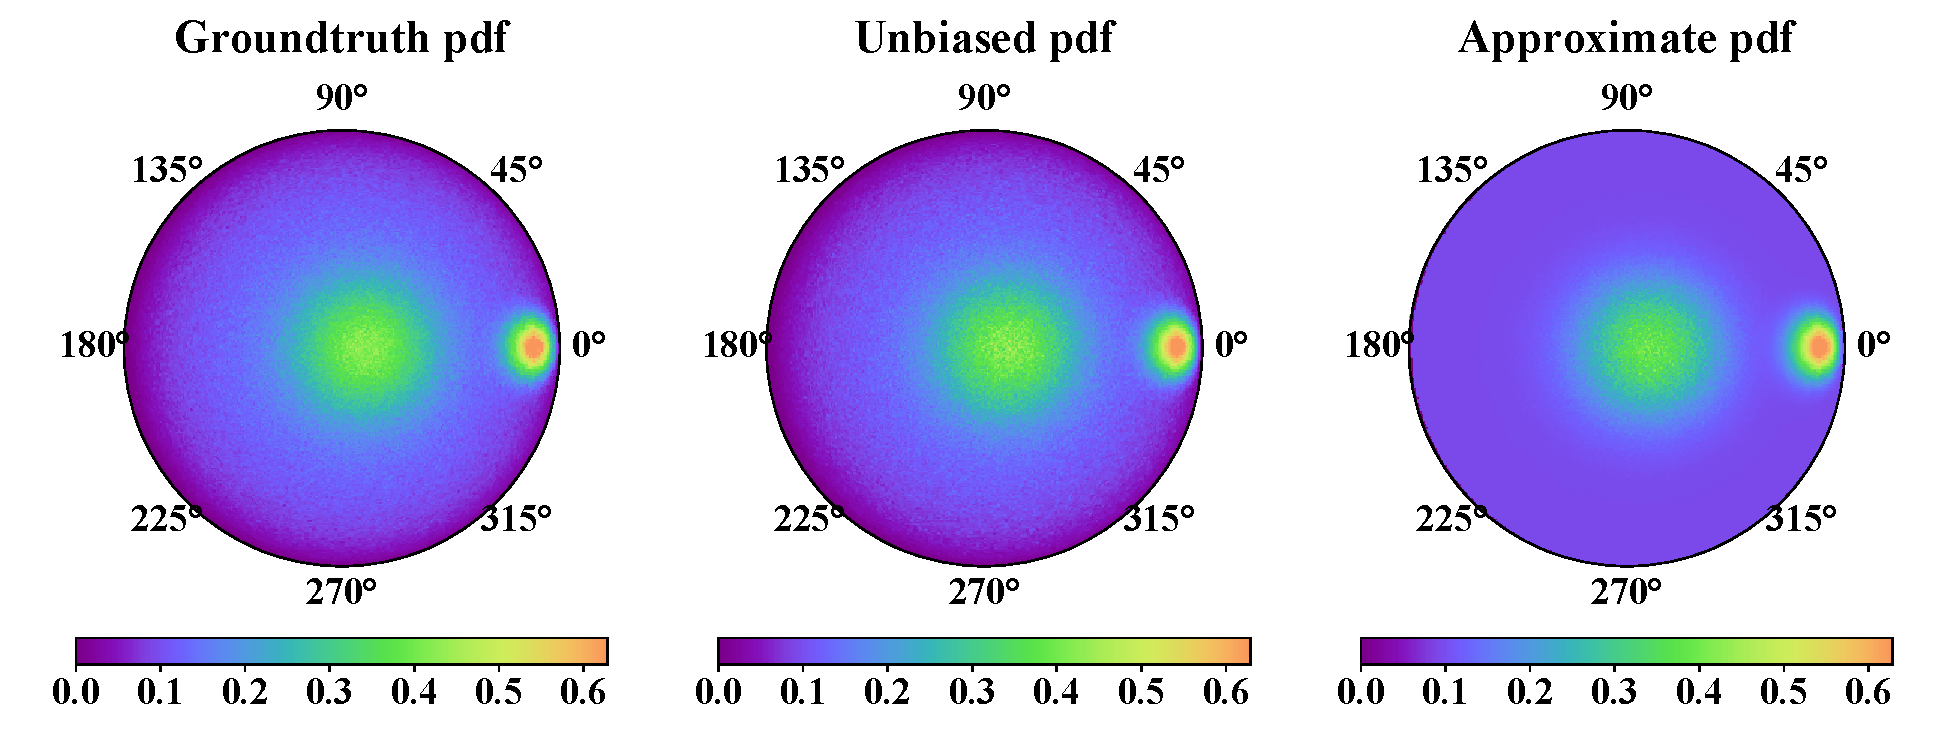
\includegraphics[width=0.65\columnwidth]{images/validations/lobe_pdf/pdf.pdf}
            \end{figure}
        \end{block}
        
        \vspace{0.5cm}
        
        \begin{block}{Comparison}
            \textbf{Equal-time comparison:}
            \vspace{-1cm}
            \begin{figure}
                \begin{tabular}{cccccc}
            		\begin{overpic}[width=0.16\textwidth]{images/validations/compare1/plane_fullsim_ref_3_2h.jpg} 
                		%\put(2,3){\bfseries \color{white} \Large } 
                	\end{overpic} &
            		\begin{overpic}[width=0.16\textwidth]{images/validations/compare1/plane_10s_pt_98spp.jpg} 
            		\put(2,3){\bfseries \color{white} \small{98 spp}} 
            		\end{overpic} &
            		\begin{overpic}[width=0.16\textwidth]{images/validations/compare1/plane_10s_bdpt_35spp.jpg} 
            		\put(2,3){\bfseries \color{white} \small{35 spp}} 
            		\end{overpic} &
            		\begin{overpic}[width=0.16\textwidth]{images/validations/compare1/plane_10s_mlt_280spp.jpg}
            		\put(2,3){\bfseries \color{white} \small{280 spp}} 
            		\end{overpic} &
            		\begin{overpic}[width=0.16\textwidth]{images/validations/compare1/plane_10s_uni_56spp.jpg} 
            		\put(2,3){\bfseries \color{white} \small{56 spp}} 
            		\end{overpic} &
            		\begin{overpic}[width=0.16\textwidth]{images/validations/compare1/plane_10s_bi_26spp.jpg} 
            		\put(2,3){\bfseries \color{white} \small{26 spp}} 
            		\end{overpic}
            		\\
            		\begin{overpic}[width=0.16\textwidth]{images/validations/compare1/plane_fullsim_ref_4_8h.jpg} 
            			%\put(2,3){\bfseries \color{white} \Large } 
            		\end{overpic} &
            		\begin{overpic}[width=0.16\textwidth]{images/validations/compare1/plane_10s_pt_60spp.jpg} 
            		\put(2,3){\bfseries \color{white} \small{60 spp}} 
            		\end{overpic} &
            		\begin{overpic}[width=0.16\textwidth]{images/validations/compare1/plane_10s_bdpt_25spp.jpg} 
            		\put(2,3){\bfseries \color{white} \small{25 spp}} 
            		\end{overpic} &
            		\begin{overpic}[width=0.16\textwidth]{images/validations/compare1/plane_10s_mlt_80spp.jpg} 
            		\put(2,3){\bfseries \color{white} \small{80 spp}} 
            		\end{overpic} &
            		\begin{overpic}[width=0.16\textwidth]{images/validations/compare1/plane_10s_uni_15spp.jpg} 
            		\put(2,3){\bfseries \color{white} \small{15 spp}} 
            		\end{overpic} &
            		\begin{overpic}[width=0.16\textwidth]{images/validations/compare1/plane_10s_bi_19spp.jpg} 
            		\put(2,3){\bfseries \color{white} \small{19 spp}}
            		\end{overpic}
            		\\
            		%
            		\small{Reference} &
            		\small{PT} &
            		\small{BDPT} &
            		\small{MLT} &
            		\small{Our uni-dir} &
            		\small{Our bi-dir}
                \end{tabular}
            \end{figure}

            % \textbf{Equal-time comparisons} of our unidirectional and bidirectional approach to standard transport algorithms, on a simple flat layered configuration lit by a small area light. 
            % For standard PT, BDPT and MLT, results are all generated using 3D tracing by applying these algorithms in a simple 3D scene containing a very large slab with flat interfaces. 
            % our estimators perform similarly, but both significantly outperform path tracing, bidirectional and Metropolis transport.
            % The references are generated using standard PT with 100K spp, and all the other images are rendered in 10 seconds.
            
            \vspace{0.5cm}
            \begin{columns}[t,totalwidth=\twocolwid]
                \begin{column}{\onecolwid} 
                    \textbf{Comparison to previous work:}
                    \begin{figure}
                        \vspace{-1cm}
                    	\begin{tabular}{ccc}
                    	    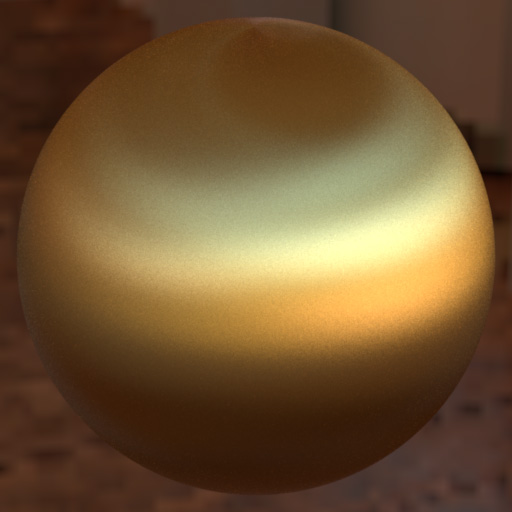
\includegraphics[width=0.32\columnwidth]{images/validations/compare2/aniso_comb_hor_hor_512spp_17min.jpg} &
                    	    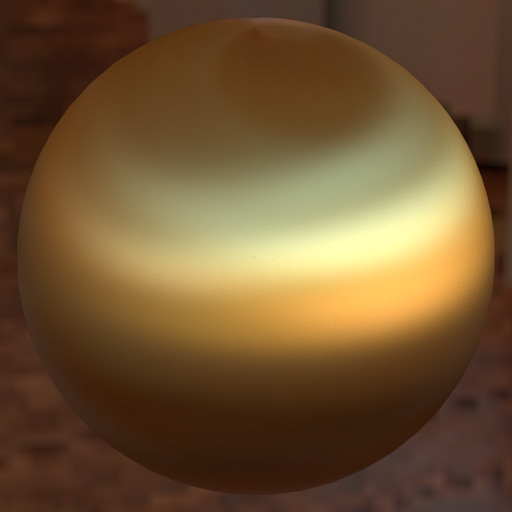
\includegraphics[width=0.32\columnwidth]{images/validations/compare2/aniso_comb_hor_hor_wenzel.jpg} &
                    	    
\includegraphics[width=0.32\columnwidth]{images/validations/compare2/na.pdf} \\
                    
                    	    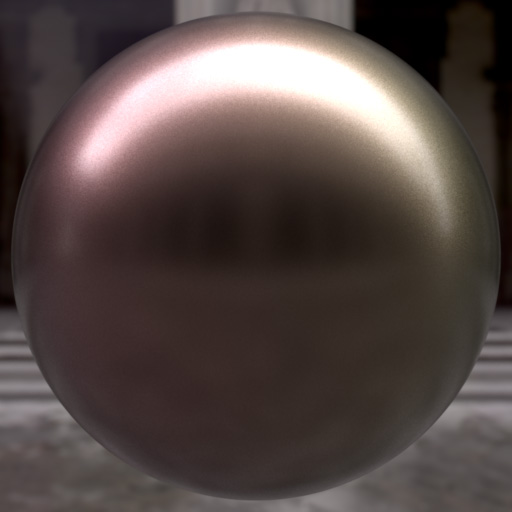
\includegraphics[width=0.32\columnwidth]{images/validations/compare2/sphere_layered_1024spp_37min.jpg} &
                    	    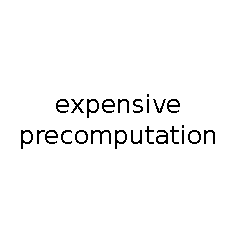
\includegraphics[width=0.32\columnwidth]{images/validations/compare2/na2.pdf} &
                    	    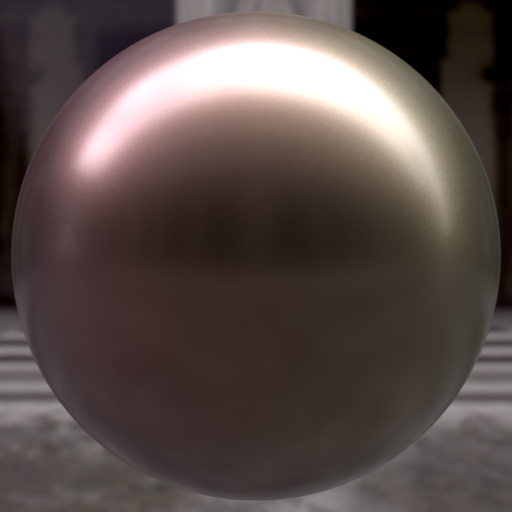
\includegraphics[width=0.32\columnwidth]{images/validations/compare2/sphere_laurent_1024spp_1_5min.jpg} \\
                    
                    	    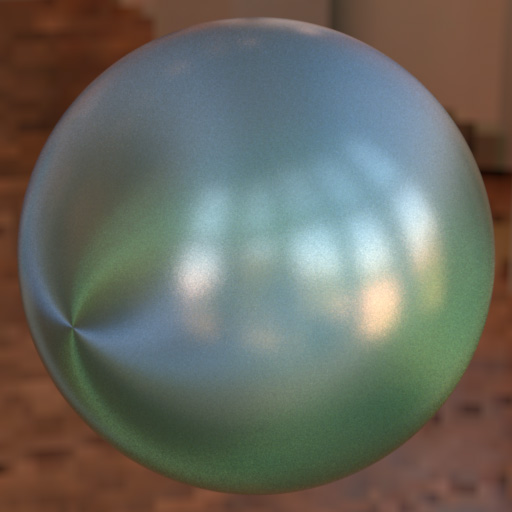
\includegraphics[width=0.32\columnwidth]{images/validations/compare2/sphere_1024spp_60min.jpg} &
                    	    
\includegraphics[width=0.32\columnwidth]{images/validations/compare2/na.pdf} &
                    	    
\includegraphics[width=0.32\columnwidth]{images/validations/compare2/na.pdf} \\
                    
                    	    \small{Ours} &
                    	    \small{[Zeltner 2018]} &
                    	    \small{[Belcour 2018]}
                    	\end{tabular}
                    \end{figure}
                \end{column}
            
                \begin{column}{\onecolwid}
                    \textbf{Comparison to volumetric cloth:}
                    \begin{figure}
                        \vspace{-1cm}
                    	\begin{tabular}{cc}
                    		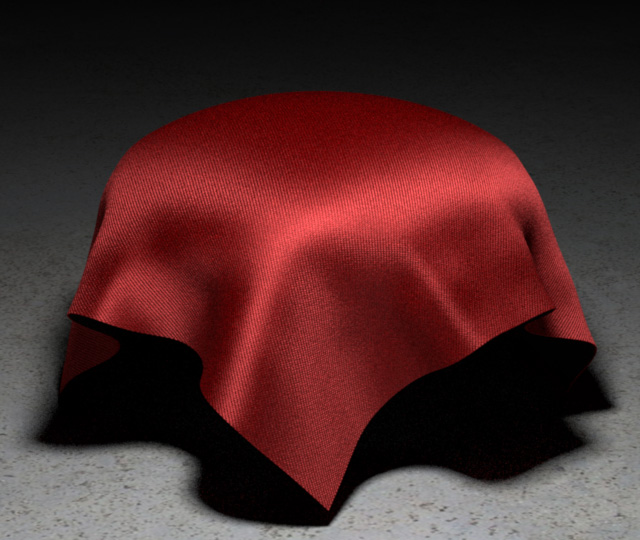
\includegraphics[width=0.49\textwidth]{images/results/gabardine_ref.jpg} &
                    		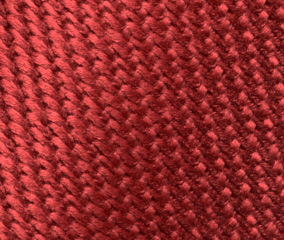
\includegraphics[width=0.49\textwidth]{images/results/gabardine_ref_inset_128spp.jpg} \\
                    		\multicolumn{2}{c}{\vspace{1cm} \small{Volume rendering}} \\
                    		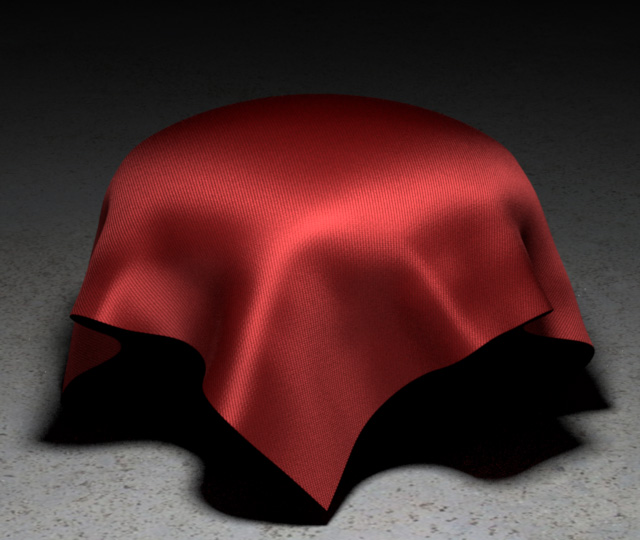
\includegraphics[width=0.49\textwidth]{images/results/gabardine.jpg} &
                    		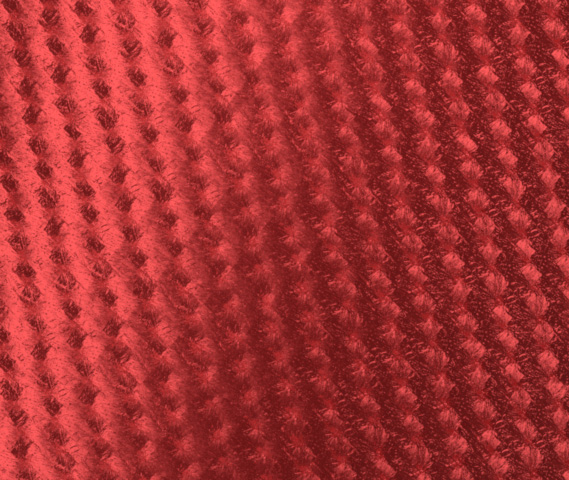
\includegraphics[width=0.49\textwidth]{images/results/gabardine_inset_512spp.jpg} \\
                    		\multicolumn{2}{c}{\small{Our BSDF + fiber-direction map}}
                    	\end{tabular}
                    \end{figure} 
                \end{column}
            \end{columns}
        \end{block}
    \end{column}
    
    %----------------------------------------------------------------------------
    %	RIGHT
    %----------------------------------------------------------------------------
    \begin{column}{\sepwid}\end{column} % Empty spacer column
    \begin{column}{\twocolwid} % The third column
        \begin{block}{More results}
            \textbf{Transmission (Spectrally varying optical densities):}
            \vspace{-1cm}
            \begin{figure}
            	\begin{tabular}{cccc}
            		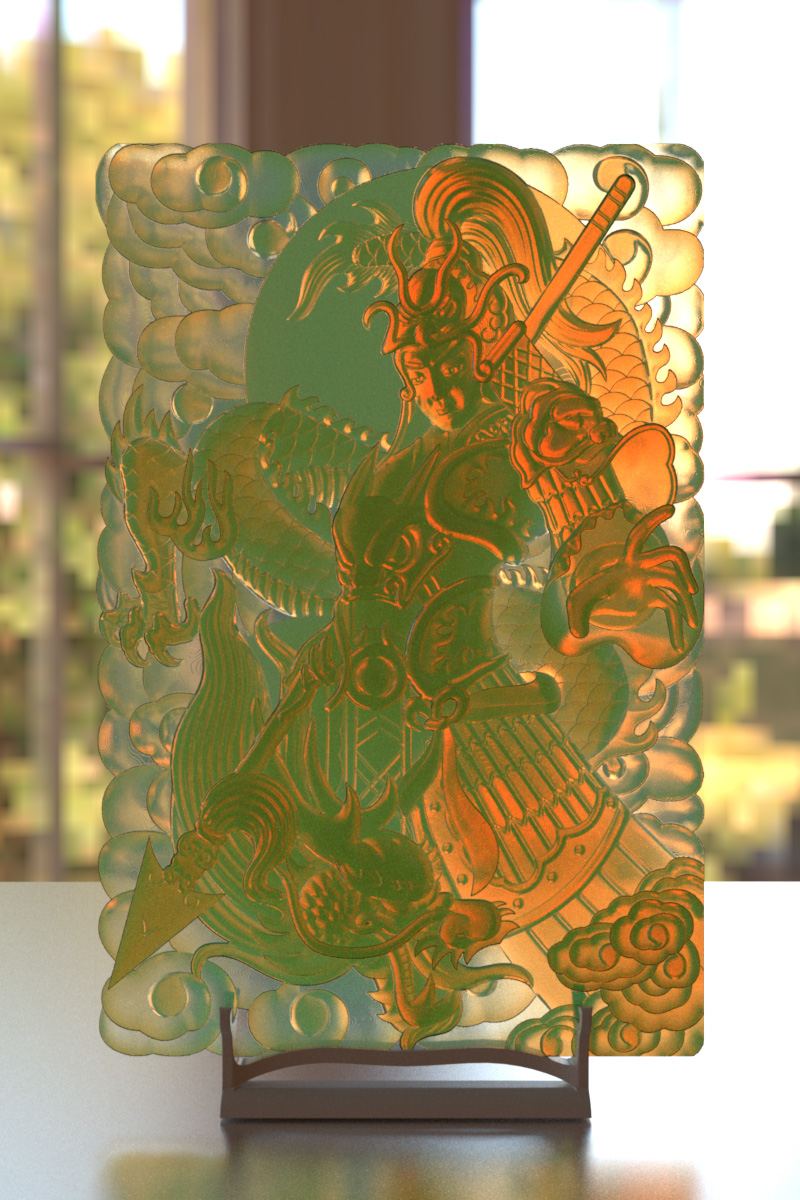
\includegraphics[width=0.24\textwidth]{images/results/zhaoyun_bg1_1.jpg} &
            		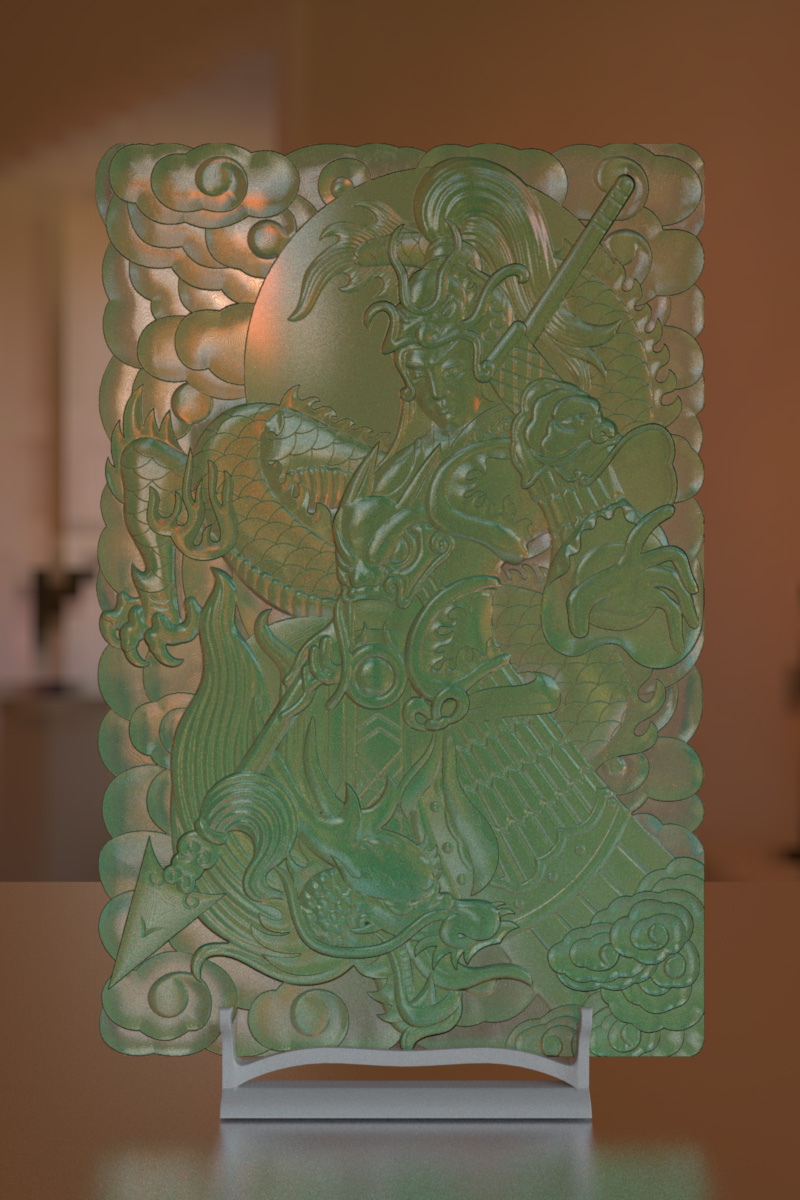
\includegraphics[width=0.24\textwidth]{images/results/zhaoyun_bg1_2.jpg} &
            		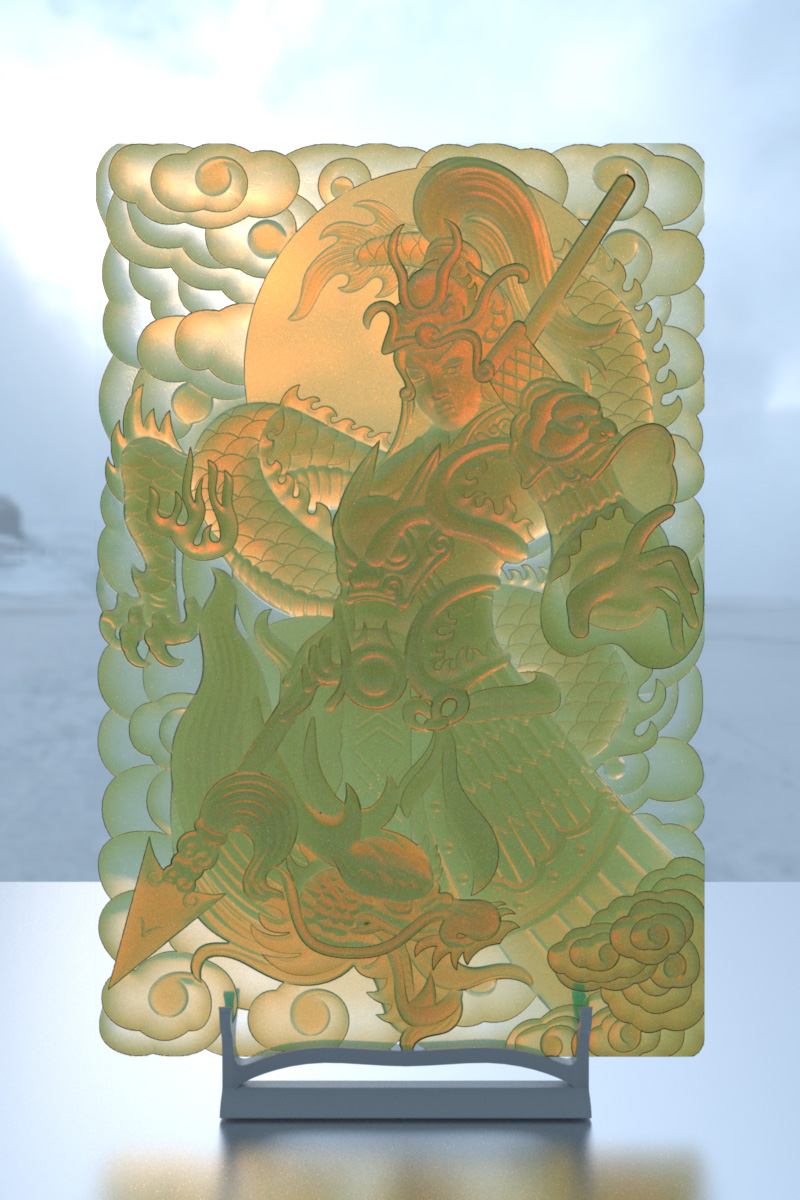
\includegraphics[width=0.24\textwidth]{images/results/zhaoyun_bg2_1.jpg} &
            		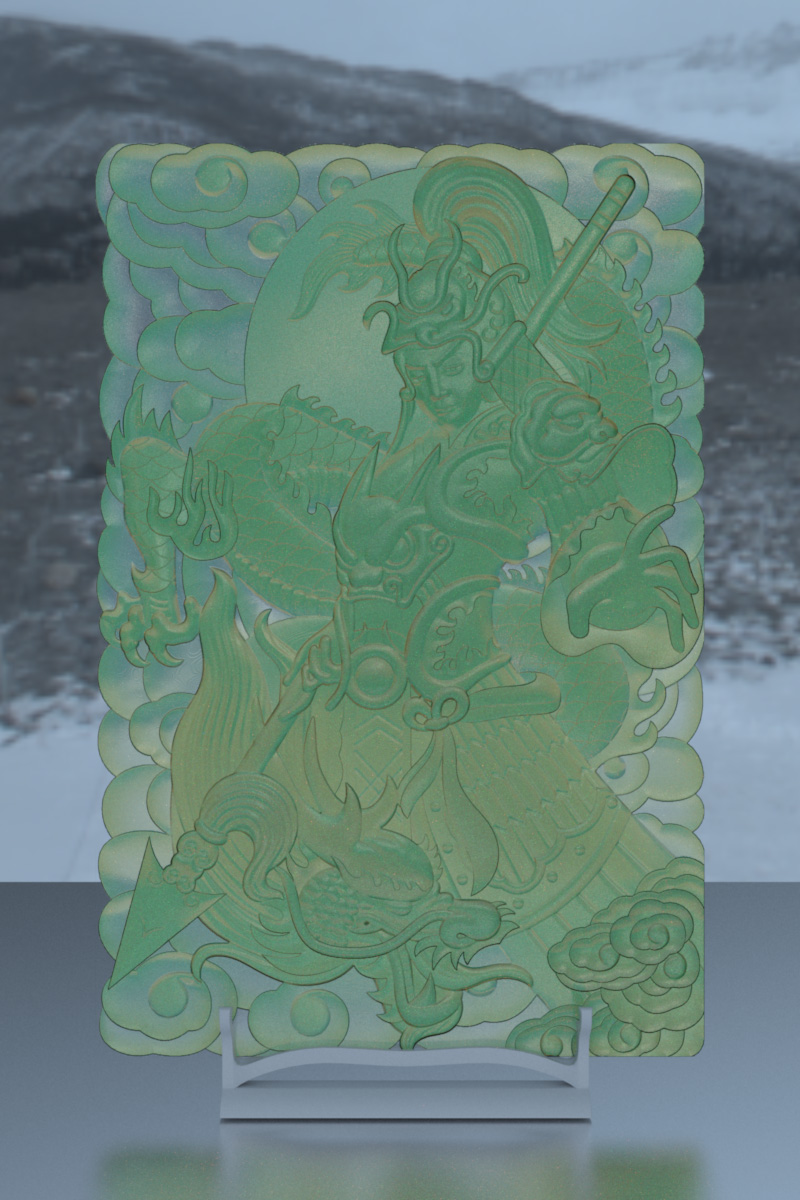
\includegraphics[width=0.24\textwidth]{images/results/zhaoyun_bg2_2.jpg}
            	\end{tabular}
            \end{figure}
            \vspace{0.5cm}
            \textbf{Transmission (Different phase function):}
            \begin{figure}
            	\begin{tabular}{cccc}
            		\begin{overpic}[width=0.24\textwidth]{images/results/magnify_g9.jpg} 
            		    \put(2,2){\bfseries \color{black} \small HG ($g = 0.9$)}
            		\end{overpic}
            		&
            		\begin{overpic}[width=0.24\textwidth]{images/results/magnify_g99.jpg} 
            		    \put(2,2){\bfseries \color{black} \small HG ($g = 0.99$)}
            		\end{overpic}
            		&
            		\begin{overpic}[width=0.24\textwidth]{images/results/magnify_vmf10.jpg} 
            		    \put(2,2){\bfseries \color{black} \small vMF ($\kappa = 10$)}
            		\end{overpic}
            		&
            		\begin{overpic}[width=0.24\textwidth]{images/results/magnify_vmf100.jpg}
                		\put(2,2){\bfseries \color{black} \small vMF ($\kappa = 100$)}
                	\end{overpic}
            	\end{tabular}
            \end{figure}
            \vspace{0.5cm}
            \textbf{Anisotropic media within layers:}
            \begin{figure}
            	\begin{tabular}{ccc}
            		\begin{overpic}[width=0.32\textwidth]{images/results/satin_spp128.jpg}
            			\put(2,60){\bfseries \color{white} \small Satin}
            		\end{overpic}
            		&
            		\begin{overpic}[width=0.32\textwidth]{images/results/twill_128spp.jpg}
            			\put(2,60){\bfseries \color{white} \small Twill}
            		\end{overpic}
            		&
            		\begin{overpic}[width=0.32\textwidth]{images/results/velvet_spp128.jpg}
            			\put(2,60){\bfseries \color{white} \small Velvet}
            		\end{overpic}
            	\end{tabular}
            \end{figure}
            \vspace{0.5cm}
            \textbf{Multi-layer BSDF:}
            \begin{figure}
            	\begin{tabular}{ccc}
            		\begin{overpic}[width=0.32\textwidth]{images/results/kettle_drop.jpg}
            			\put(2,3){\bfseries \color{white} \small}
            		\end{overpic}
            		&
            		\begin{overpic}[width=0.32\textwidth]{images/results/kettle_logo.jpg}
            			\put(2,3){\bfseries \color{white} \small}
            		\end{overpic}
            		&
            		\begin{overpic}[width=0.32\textwidth]{images/results/kettle_all.jpg}
            			\put(2,3){\bfseries \color{white} \small}
            		\end{overpic}
            	\end{tabular}
            \end{figure}
        \end{block}

        \begin{block}{References}
            % [1] Tizian Zeltner and Wenzel Jakob. \textbf{"The layer laboratory: A calculus for additive and subtractive composition ofanisotropic surface reflectance."} \textit{ACM Trans. Graph., 2018.} \\ 
            % [2] Laurent Belcour. \textbf{Efficient rendering of layered materials using an atomic decomposition withstatistical operators."} \textit{ACM Trans. Graph., 2018.}\\
            \vspace{-1cm}
            \nocite{*} % Insert publications even if they are not cited in the poster
            \bibliographystyle{unsrt}
            \bibliography{references.bib}
        \end{block}
    \end{column} % End of the third column
    
\end{columns} % End of all the columns in the poster

\begin{tikzpicture}[remember picture,overlay] 
\node [shift={(-5cm,-87cm)}] at (current page.north east) {
\includegraphics[height=7cm]{images/logo/qr-code.png}}; 
\end{tikzpicture}

\end{frame} % End of the enclosing frame
\end{document}